%%%%%%%%%%%%%%%%%%%%%%%%%%%%%%%%%%%%%%%%%
% Class Notes Template
% LaTeX Template
% By: Ryan Grove
%%%%%%%%%%%%%%%%%%%%%%%%%%%%%%%%%%%%%%%%%

%----------------------------------------------------------------------------------------
%	PACKAGES AND OTHER DOCUMENT CONFIGURATIONS
%----------------------------------------------------------------------------------------

\documentclass[paper=a4, fontsize=11pt]{scrartcl} % A4 paper and 11pt font size

\usepackage[T1]{fontenc} % Use 8-bit encoding that has 256 glyphs
\usepackage{fourier} % Use the Adobe Utopia font for the document - comment this line to return to the LaTeX default
\usepackage[english]{babel} % English language/hyphenation
\usepackage{amsmath,amsfonts,amsthm} % Math packages

\usepackage{lipsum} % Used for inserting dummy 'Lorem ipsum' text into the template

\usepackage{sectsty} % Allows customizing section commands
\allsectionsfont{\centering \normalfont\scshape} % Make all sections centered, the default font and small caps

\usepackage{fancyhdr} % Custom headers and footers
\pagestyle{fancyplain} % Makes all pages in the document conform to the custom headers and footers
\fancyhead{} % No page header - if you want one, create it in the same way as the footers below
\fancyfoot[L]{} % Empty left footer
\fancyfoot[C]{} % Empty center footer
%\fancyfoot[R]{\thepage} % Page numbering for right footer
\renewcommand{\headrulewidth}{0pt} % Remove header underlines
\renewcommand{\footrulewidth}{0pt} % Remove footer underlines
\setlength{\headheight}{13.6pt} % Customize the height of the header

\numberwithin{equation}{section} % Number equations within sections (i.e. 1.1, 1.2, 2.1, 2.2 instead of 1, 2, 3, 4)
\numberwithin{figure}{section} % Number figures within sections (i.e. 1.1, 1.2, 2.1, 2.2 instead of 1, 2, 3, 4)
\numberwithin{table}{section} % Number tables within sections (i.e. 1.1, 1.2, 2.1, 2.2 instead of 1, 2, 3, 4)

\setlength\parindent{0pt} % Removes all indentation from paragraphs - comment this line for an assignment with lots of text

\usepackage{lastpage}
\usepackage{fancyhdr}
\cfoot{\thepage\ of \pageref{LastPage}}

\def\v{\hbox{$\mathbf v$}}
\def\w{\hbox{$\mathbf w$}}
\def\u{\hbox{$\mathbf u$}}
\def\x{\hbox{$\textbf{x}$}}
\def\z{\hbox{$\mathbf z$}}
\def\a{\hbox{$\mathbf a$}}
\def\b{\hbox{$\mathbf b$}}
\def\L{\hbox{$\mathcal L$}}
\def\C{\hbox{$\mathbb C$}}
\def\B{\hbox{$\mathcal B$}}
\def\R{\hbox{$\mathbb R$}}
\def\X{\hbox{$\underline X$}}
\def\Q{\hbox{$\mathbb Q$}}
\def\R{\hbox{$\mathbb R$}}
\def\N{\hbox{$\mathbb N$}}
\def\C{\hbox{$\mathbb C$}}
\def\0{\hbox{$\mathbf 0$}}
\def\Y{\hbox{$\underline Y$}}
\def\a{\hbox{$\mathbf a$}}
\def\u{\hbox{$\mathbf u$}}
\def\w{\hbox{$\mathbf w$}}
\def\y{\hbox{$\mathbf y$}}
\def\X{\hbox{$\underline X$}}
\def\dd{\hbox{$\partial $}}
\def\B{\hbox{$\mathcal B$}}
\def\F{\hbox{$\mathcal F$}}
\def\L{\hbox{$\mathcal L$}}
\def\M{\hbox{$\mathcal M$}}
\def\D{\hbox{$\mathscr {D}$}}
\def\RR{\hbox{$\mathscr{R}$}}
\def\I{\hbox{$\mathcal I$}}

\usepackage{amssymb}
%\theoremstyle{plain}
\usepackage[margin = .75in]{geometry}
\newtheorem{claim}{Claim}
\newtheorem{theorem}{Theorem}[section]
\newtheorem{lemma}[theorem]{Lemma}
\newtheorem{proposition}[theorem]{Proposition}
\newtheorem{corollary}[theorem]{Corollary}
\newtheorem{problem}[theorem]{Problem}
%\theoremstyle{definition}
\newtheorem{definition}[theorem]{Definition}
%\theoremstyle{remark}
\newtheorem{remark}[theorem]{Remark}
\newtheorem{remarks}[theorem]{Remarks}
\newtheorem{example}[theorem]{Example}
\newcommand{\ds}{\displaystyle}
\newcommand{\ZZ}{\mathbb{Z}}
\newcommand{\QQ}{\mathbb{Q}}
\newcommand{\e}{\varepsilon}
\newcommand{\bbf}{\textbf}
\newcommand{\p}{\parallel}
\usepackage{color}
\newcommand{\field}[1]{\mathbb{#1}}
\usepackage{amsmath}
\usepackage{amsthm}
\usepackage{amssymb}
\usepackage{mathrsfs}
\usepackage{cancel}
\usepackage{upgreek}
\usepackage{graphicx}
\usepackage{multirow}
\usepackage{setspace}
\usepackage{url}
\usepackage{subfigure}
\usepackage{enumerate}
\usepackage{cases}
\usepackage{mathrsfs}
\usepackage{rotating}

%----------------------------------------------------------------------------------------
%	TITLE SECTION
%----------------------------------------------------------------------------------------

\newcommand{\horrule}[1]{\rule{\linewidth}{#1}} % Create horizontal rule command with 1 argument of height

\title{	
\normalfont \normalsize 
\textsc{Ryan Grove, Clemson University, MATH1080 - 9} \\ [25pt] % Your name, university, class
\horrule{0.5pt} \\[0.4cm] % Thin top horizontal rule
\huge Section 7.5: Strategy for Integration \\ % The assignment title
\horrule{2pt} \\[0.5cm] % Thick bottom horizontal rule
}

\author{Date:} % The due date

\date{\normalsize January ???, 2016} % A custom date

\begin{document}

\maketitle % Print the title

\begin{flushleft}
\begin{tabular}{l l}
Name: \rule{3.2in}{.01cm}  & {}%Table number: \rule{1in}{.01cm}\\
\end{tabular}
\end{flushleft}

%----------------------------------------------------------------------------------------
%	Lecture
%----------------------------------------------------------------------------------------

\section*{\textbf{Lecture:}}

This section presents a collection of miscellaneous integrals in random order where the main challenge is to recognize which technique or formula to use.\\
\indent

\[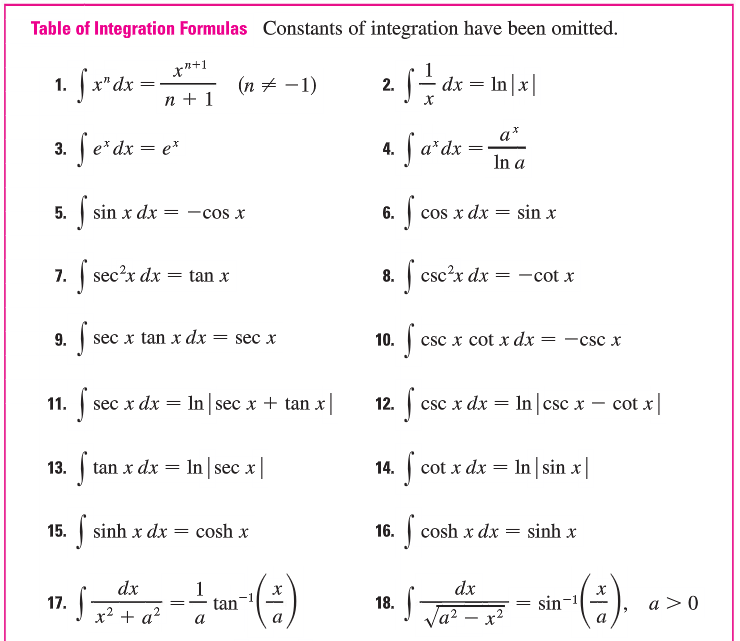
\includegraphics[scale=.5]{7-5pic1.png}\]
\indent\\

\newpage
\section*{Four-Step Strategy}
\begin{enumerate}
\item[\textbf{1.}] \textbf{Simplify the Integrand if Possible.} Use algebraic manipulation or trig identities.\\
Sometimes the use of algebraic manipulation or trigonometric identities will simplify the integrand and make the method of integration obvious. For example:\\
\indent
\begin{align*}
\ds\int \sqrt{x}(1+\sqrt{x})dx &= \ds\int (\sqrt{x} + x)dx\\
 \\
\ds\int \ds\frac{\tan\theta}{\sec^2\theta}d\theta &= \ds\int \ds\frac{\sin\theta}{\cos\theta}\cos^2\theta d\theta\\
&= \ds\int \sin \theta \cos \theta d\theta\\
&= \ds\frac{1}{2} \ds\int \sin 2\theta d\theta\\
\\
\ds\int (\sin x + \cos x)^2 &= \ds\int (\sin^2 x + 2\sin x \cos x + \cos^2 x)dx\\
&= \ds\int (1+2\sin x\cos x)dx\\
\end{align*}
\indent

\item[\textbf{2.}] \textbf{Look for an Obvious U-Substitution.}
% Try to find some function $u=g(x)$ in the integrand whose differential $du=g'(x)dx$ also occurs, apart from a constant factor. For example:\\
%
%\[\text{In the integral, } \ds\int \ds\frac{x}{x^2-1}dx

\item[\textbf{3.}] \textbf{Classify the Integrand According to Its Form.}
\begin{enumerate}
\item[(a)] \textit{Trigonometric functions}\\
\item[(b)] \textit{Rational functions} $\implies$ PFD\\
\item[(c)] \textit{Integration by Parts}\\
\item[(d)] \textit{Radicals}\\
\begin{enumerate}
\item[(i)] If $\ds\sqrt{\pm x^2 \pm a^2}$ occurs, use a trigonomentric substitution.
\item[(ii)] If $\sqrt[n]{ax+b}$ occurs, use the rationalizing subsitution $u=\sqrt[n]{ax+b}$.\\
 More generally, this sometimes works for $\sqrt[n]{g(x)}$.\\
\end{enumerate}
\end{enumerate}

\item[\textbf{4.}] \textbf{Try Again.} Remember, the first approach you choose might not be the correct or easiest, so if it does not appear to work, try something else:\\
\begin{enumerate}
\item[(a)] \textit{Try substitution.} Try something that maybe isn't so obvious.\\
\item[(b)] \textit{Try parts.} Although mostly used on products of different functions, IBP is sometimes effective on single functions such as inverse trig or log functions.\\
\item[(c)] \textit{Manipulate the integrand.} Multiplying by the conjugate might help as in the following example:
\begin{align*}
\ds\int\ds\frac{dx}{1-\cos x} &= \ds\int \ds\frac{1}{1-\cos x }\cdot \ds\frac{1+\cos x}{1+\cos x} dx = \ds\int \ds\frac{1+\cos x}{1-\cos^2 x}dx\\
&= \ds\int \ds\frac{1+\cos x}{\sin^2 x}dx = \ds\int\left(\csc^2 x + \ds\frac{\cos x}{\sin^2 x}\right) dx.
\end{align*}
\item[(d)] \textit{Relate the problem to previous problems.}\\
\item[(e)] \textit{Use several methods} Sometimes more than one method is required to evaluate an integral.\\
\end{enumerate}

\section*{Can We Integrate All Continuous Functions?}

The answer is $\underline{\hspace{0.5in}}$. At least not in terms of the functions that we are familiar with. No matter how hard we try we will never succeed in evaluating 
\[\ds\int e^{x^2} dx\]
in terms of the functions we know. (In Chapter 11, however, we will see how to express $\ds\int e^{x^2} dx$ as an infinite series.) The same can be said of the following integrals:

\[\begin{array}{rlll}
&\ds\int \ds\frac{e^x}{x}dx \hspace{1in}  &\ds\int \sin(x^2)dx \hspace{1in} & \ds\int \cos(e^x)dx\\
&\ds\int \ds\sqrt{x^3+1}dx \hspace{1in} & \ds\int \ds\frac{1}{\ln x}dx \hspace{1in} & \ds\int \ds\frac{\sin x}{x} dx\\
\end{array}\]
\indent



\end{enumerate}
%\fbox{
%  \parbox{\textwidth}{
%  \vspace{5pt}

















%----------------------------------------------------------------------------------------

\end{document}